%
\chapter{Implementation}\label{cha:Implementation}
%
\section{Test Track}\label{sec:Test Track}

As previously mentioned, the medium-term goal of this master thesis is attending the Carola-Cup at Braunschweig University, so the test truck was prepared according to the Carola-Cup criteria by Nicolas Acero Sepulveda, who also did his bachelor thesis with this model automobile. For this test truck, two black PVC floor carpets were used and on these floor carpets, the lanes of the track were made by using white electrical tape. The straight part of the track was made on one of these PVC floor carpets and the curved part of track was made on the second PVC floor carpet. The straight part of the track is approximately 2 meters long and the curve radius of the curved part of test track is approximately 1 meter. This curve is the tightest curve at Carola-Cup, so with this, the test track can be tested in the worst case scenario. In the Carola-Cup competition, the track is much larger; however, for the purposes of this master thesis, a larger test track in not needed.

\begin{figure}[H]
	\centering
	\hspace*{0cm}   
	\includegraphics[width=150mm,scale=1]{./Bilder/Test Truck.jpg}
	\caption{Test Truck}
\end{figure}

%
\section{Hardware}\label{sec:Hardware}



%
\subsection{Model Auto}\label{sec:Model Auto}


During the course of this master thesis, a model automobile was being used which was prepared for the Projectseminar 
Echtzeitsysteme at Technical University of Darmstadt. The chassis, steering mechanism, power train, and engine control 
were derived from the model-building of a Japanese company, Tamiya. The maximum velocity of the model automobile is 
approximately 1 m/s and the minimum steering radius is around 90 cm. 

\begin{figure}[H]
	\centering
	\hspace*{0cm}   
	\includegraphics[width=150mm,scale=1]{./Bilder/Model Auto.jpg}
	\caption{Model Auto}
\end{figure}

%
\subsection{Microcontroller and Main Board}\label{sec:Microcontroller and Main Board}


In this model auto, there is a microcontroller and a main board. The microcontroller is used for controlling steering 
and receiving the measurements from ultrasonic sensors and hall effect sensors. The 16-bit microcontroller is from 
MB96300 series from Fujitsu company.

The main board on the model car is from PD10BI-MT ThinMini-ITX series from MiTAC company. This main board communicate 
with the microcontroller over via UART interface through USB connection. On this main board, there is an Intel 
Quadcore-Processor and an Intel HD Graphics card. Furthermore, there is a 8 GB DDR3-1600 RAM and 1Gbit/s Ethernet, VGA, HDMI, USB 2.0/3.0, SATA ports and an Intel Dual Band Wireless AC 7260 Network adapter, which is connected to two external WLAN antennas. A 60 GB Kingston SSD-Harddisk is connected over an integrated PCI-Express Port. A 3200 mAh Li-Fe battery is used as power supply.
%

\subsection{Camera}\label{sec:Camera}


The camera is one of the main components of lane detection and accordingly, autonomous driving. For this thesis, I had 
to research the most suitable camera because all cameras have different properties.

At the beginning of the Projectseminar Echtzeitsysteme, the Logitech C270 HD Webcam was being used. The resolution of 
the camera is 1280x960 pixels and the Frame per Second (FPS) value is 30 Hertz (Hz) at a 640x480 pixel resolution. 
The field of View (FOV) is just 60 degrees. The problem with this camera is that if there is a curve, the camera 
cannot see all of the lanes, and thus is not very suitable for lane detection. When I started my master thesis, there 
was a Kinect v2 camera on the model car.  The Kinect v2 camera was developed by Microsoft and released in 2013. This 
camera has a depth sensor with a resolution of 512x424 pixels and its FOV is 70x60 degrees. The FPS value is 30 Hz at 
a 512x424 pixel resolution. This camera also has a color camera with resolution of 1920x1080 pixels and a FOV of 
84.1x53.8 degrees. The FPS value is 30 Hz at a 1920x1080 pixel resolution. This camera had two main disadvantages for 
this master thesis. The first disadvantage is the FOV value of camera. This value is better than the value of Logitech 
C270 camera but it is still not enough for curve lane detection. The second main disadvantage is the location of the 
color camera. The color camera of this camera is not in the middle of camera, but rather, on the right. This is a 
disadvantage for us because when there are curves going left as opposed to right, the camera is unable to see the 
left and even perhaps the middle lane of the truck. Thus, this is problematic for lane detection.

Due to these reasons, I had to choose a camera which has a sufficiently high FOV value. After doing research, I decided 
that the Genius Widecam F100 camera is the best choice for this master thesis because this camera has a FOV value of 
120 degrees and it can also be used with the Linux Operating System. The resolution of this camera is 1920x1080 pixels 
and the FOV value is 120 degrees. The FPS is 30 Hz at a 1920x1080 pixel resolution. With this camera, it is possible 
to detect most if not all lanes, including when there are curves. 

\begin{figure}[H]
	\centering
	\hspace*{0cm}   
	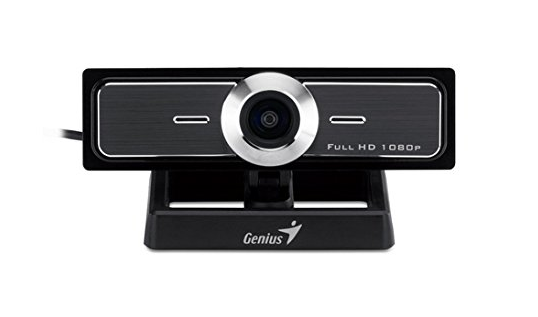
\includegraphics[width=150mm,scale=1]{./Bilder/Genius_F100_camera.png}
	\caption{Genius 120-degree Ultra Wide Angle Full HD Conference Webcam(WideCam F100) }
\end{figure}


%
\section{Software}\label{sec:Software}


In this chapter, the software algorithms will be focused, which are defined in this master thesis.  Through program flow charts and explaination of all steps of program flow charts, it will be tried to explain algorithms better. For finding the best solution, 5 different source codes versions(?variants/?methods) were generated. For all these source codes,the computing times were calculated and compared which solution can detect the lanes better. In next pages, there are detailed explanations of used versions(?variants/?methods). The development environment and the used softwares will be also described , which are used in master thesis.

%
\subsection{Development Environment and Related Softwares}
\label{sec:Development Environment and Related Softwares}

As also mentioned at subsection \ref{sec:Microcontroller and Main Board}, in this project the introduced main board was used. One of the compact and fast version of Linux 16.04 operating system, \textit{Lubuntu} was installed in this main board.

The version \textit{Kinetic} of ROS was used for implementation of this master thesis. ROS is the abbreviation of \textbf{R}obotic \textbf{O}perating \textbf{S}ystem, which is a robotics middleware (i.e. collection of software frameworks for robot software development). At ROS wiki page\cite{ROS}, ROS is defined that, ROS is an open-source, meta-operating system for your robot. It provides the services you would expect from an operating system, including hardware abstraction, low-level device control, implementation of commonly-used functionality, message-passing between processes, and package management. It also provides tools and libraries for obtaining, building, writing, and running code across multiple computers.

For using prepaid image processing functions, an open source computer vision and machine learning software library was used, which is called as OpenCV. According to OpenCV website\cite{OpenCV}, there are more than 2500 optimized algorithms in OpenCV library and OpenCV has more than 47 thousand people of user community.

ROS can be programmed by programming languages Python, C++ or Lisp and OpenCV can be programmed by programming languages Python or C++. In this master thesis, C++ was used.

%
\subsection{Preprocessing :}\label{sec:Preprocessing}

There are so different possibilities for lane detection algorithms. Of course, each of them has some advantages and disadvantages. In this master thesis, some different methods were defined and in this chapter, these methods will be explained in detail.

In all these methods, some processes are common, which is called as preprocessing phase. At the beginning,\emph{\color{blue} the frames are gotten from the camera via ROS-Topic.} ROS uses different image formats but OpenCV uses as another image format Matrix(Mat) object. This taken frame via ROS-Topic must be converted from ROS image data type to Mat object. For that converting, a ROS-Package were used, which is called as \textit{cvbridge}\cite{cv_bridge}. cvbridge converts to ROS image format to Mat Object which is the OpenCV Image Format. 

Mat is a class which has two parts. The parts are a matrix header and a pointer to the matrix containing the pixel values. The matrix header contains the informations like the size of matrix, storing method and etc. It has always fixed size but the size of matrix is variable from image to image.

There are so many methods, which can store the pixel values to the Mat object. In this case, the color space and used data type can be choosed. For gray images, it is easy to choose the color space because there are just two colors : black and white. With changing the density of colors(black and white), it is possible to create many shades of gray. There are more methods for colorful images. Colorful images have generally three or four channels. These three channels are used for RGB color values. The RGB colors are based on red, green and blues colors which can be detected all colors by human eyes. For transparency of a color can be used a fouth channel which is calles as alpha(A).

There are also another color formats, which have some advantages\cite{OpenCV_Mat}. 

\begin{itemize}

\item RGB format is so similar to human eye use, but at OpenCV display system uses BGR format which has another row of colors than RGB format  

\item HSV and HLS formats are more natural way to describe colors. They decompose colors into their hue, saturation and value/luminance components. Another advantage of HSV and HLS make less sensitive to the light conditions of the input image.

\item At JPEG image formats is used YCrCb format.

\item if the distance of a given color to another color want to be measured, CIE L*a*b* format is more suitable than others.

\end{itemize}

After the frame from Camera via ROS-Topic was received, the colorful frame has to be converted to grayscale frame. For detection lanes, Hough Transformation is used and for Hough Transformation, grayscale format of input image is needed. To convert a frame from BGR format to grayscale format brings some advantages, the main advantage is the processing time. Normally colorful frame matrix content has three or four channels but at grayscale frame matrix content has just one channel so grayscale frame matrix size is much smaller compare to colorful frame matrix size. Because of this reason the image processing time is much more smaller at grayscale format compare to BGR format. For converting BGR formatted frame to grayscale formatted frame, \textit{cvtColor} function from OpenCV is used.

 For stabile lane detection, the light conditions must be considered. Because of this reason, after converting the frame with BGR format to grayscale format, the lightest and darkest pixels were searched. After finding the lightest and darkest pixels, light conditions can be estimated approximately. These values will be used in the next step. After this processing, a filter is applied to all frames which tranforms an image into a binary image by transforming each pixel according to whether it is inside or outside a specified range. The user chooses a threshold value to process. If a pixel is greater than this value, it is assigned an 'inside' value. Otherwise it is assigned an 'outside' value. Depending on the lightest and darkest pixel values, the threshold value changes. Through this dynamical parameter, the lanes are more clear detectable and noises can be cancelled more successful.

After threshold filter, an edge detection filter must be applied. In this master thesis, the Sobel operator is used which explained at Chapter 2 in detail.
 
 This preprocessing part is common for all cases but after this process, there are differences at cases.
 
%
\subsection{Method 1/Case 1 : Hough Transformation + Curve Fitting + IPM}\label{sec:Method 1}

When the preprocessing part is over, the lanes must be detected. For the finding the position of lanes, the Standart Hough Transformation is used. But the Standart Hough Transformation didn't used to all of the frame, the frame were cropped. This cropping has a reason and there is an advantage thanks of cropping. It will be explained soon in detail.

We get frames from camera 640x480 pixels resolution. It was the default value at that camera. The resolution of the camera can be increased by its settings, but it is not possible to decrease. For decreasing the resolution of the camera, there is another method and it is used in another case so it will be explained when it is used in another case. In this case, the minimum resolution is used, which the camera allows us. There are some reasons. The most important reasons is, if the resolution is increased, there are more pixels so the computing time increases too. High computing time is something, which we don't want to have.
 
Height of the frame has 640 pixels, but as before mentioned, the frame was cropped. As seen at Figure \ref{fig:Case1_withoutCropped}, if there is a curve, far points from camera won't be the part of truck. There can be some stuffs which are not relevant with truck and lanes so these stuffs caused to produce Standart Hough Transformation lines. In this thesis, the Standart Hough Transformation were used, if there is an edge which could detected by Sobel Operator, produces a red line so the first 100 pixels of frame height were took off and the last 540 pixels were used. As seen at Figure \ref{fig:Case1_withCropped}, the red lines are shown just last 540 pixels of frame height so they don't cover the irrelevant informations at the frame. If there is a lane, the red lines are so close each other but if there is no lane, there are so many distance(at least 50 pixels) between red lines. At Figure \ref{fig:Case1_withCropped}, there are three different groups of red lines. All these group include a lane. Thanks of Standart Hough Transformation, we know that, between which vertically pixels stand the lanes. 

\begin{figure}[H]
  \centering
  \subfloat[Original Image]{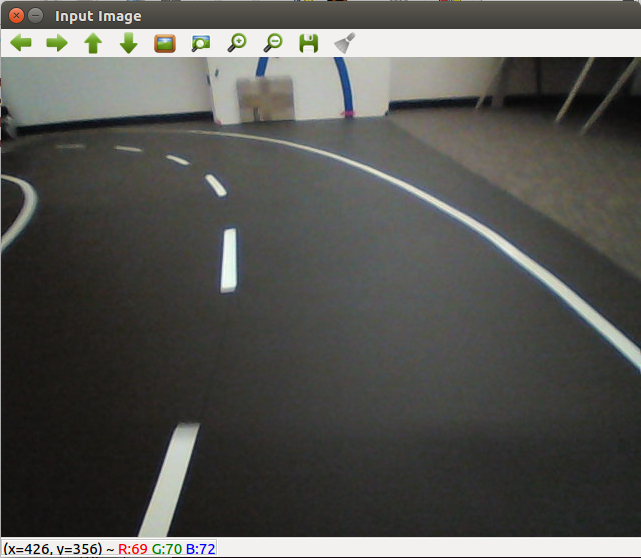
\includegraphics[width=0.3\textwidth]{./Bilder/Case1_inputImg.png}\label{fig:Case1_inputImg}}
  \hfill
  \subfloat[Hough Transformation without Cropping Image]{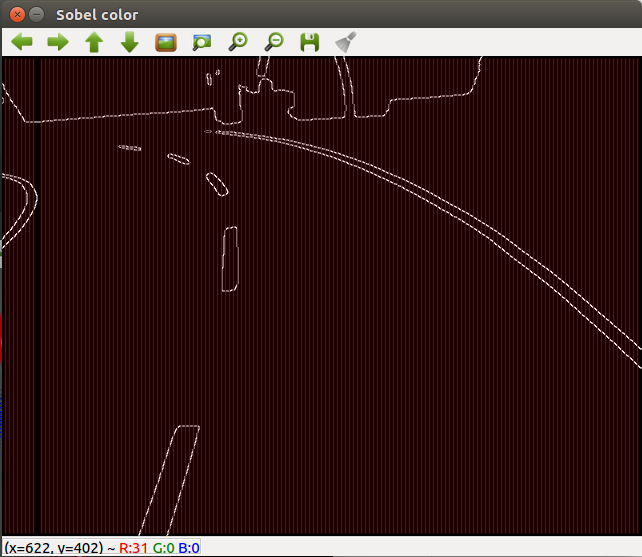
\includegraphics[width=0.3\textwidth]{./Bilder/Case1_withoutCropped.png}\label{fig:Case1_withoutCropped}}
  \hfill
  \subfloat[Hough Transformation with Cropping Image]{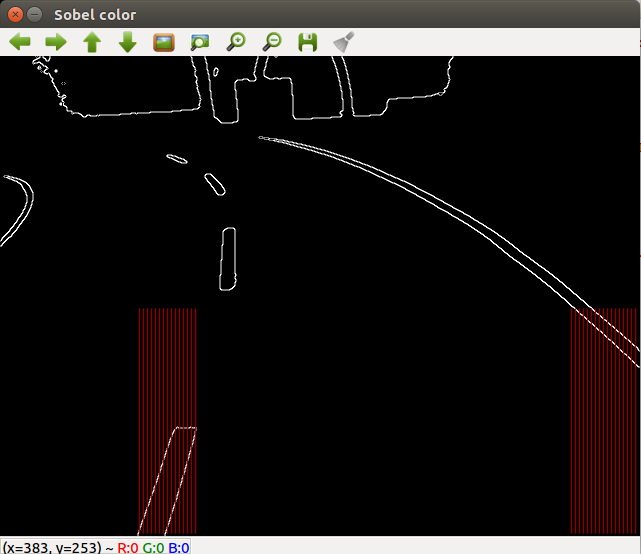
\includegraphics[width=0.3\textwidth]{./Bilder/Case1_withCropped.png}\label{fig:Case1_withCropped}}
  \caption{Detecting Lane Positions}
\end{figure}

After this processing, we have to find the starting points of lanes and the all pixels which are on the lanes. For that, we have to use Probabilistic Hough Transformation. Probabilistic Hough Transformation is a bit different than Standart Hough Transformation. Standart Hough Transformation is more suitable for straight lanes but if there is a curve, Standart Hough Transformation doesn't work enough good. As before mentioned, a line can be represented as y = mx+c or in parametric form, as $\rho$ = x $\cos \theta$ + y$ \sin \theta$ where  $\rho$ is the perpendicular distance from origin to the line, and $\theta$ is the angle formed by this perpendicular line and horizontal axis measured in counter-clockwise. But it is different at Probabilistic Hough Transformation. A line is represented by two or more points. If Probabilistic Hough Transformation finds at least two points from the same lane, it represents beginning and ending points of these lines.

In this master thesis, the lines are not shown because we don't see the Probabilistic Hough Lines. We need just these points(pixels), which are on the lanes. 

\begin{figure}[H]
  \centering
  \subfloat[Original Image with Probabilistic Hough Transformation]{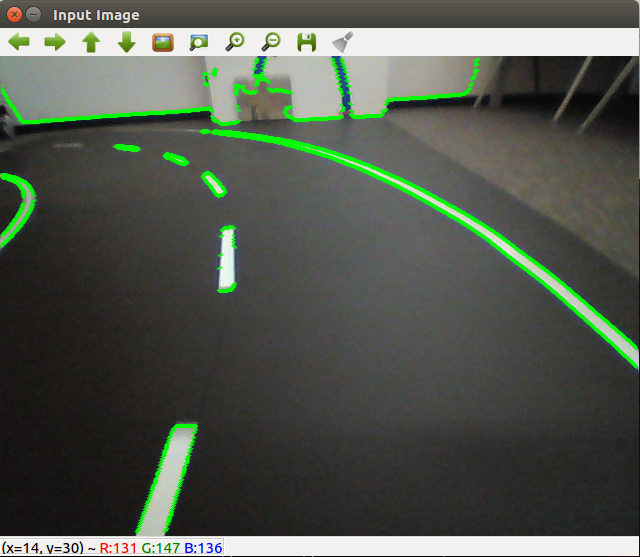
\includegraphics[width=0.45\textwidth]{./Bilder/Case1_HoughPoints_Original.png}\label{fig:Case1_HoughPoints_Original}}
  \hfill
  \subfloat[A Image with Sobel Operator and Probabilistic Hough Transformation]{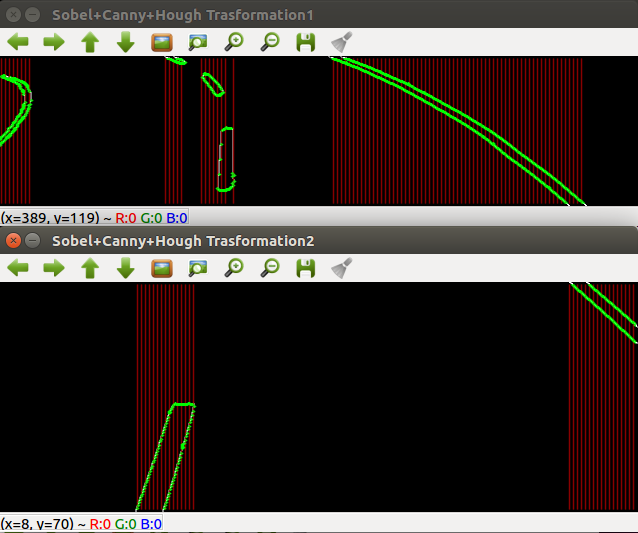
\includegraphics[width=0.45\textwidth]{./Bilder/Case1_HoughPoints_Sobel.png}\label{fig:Case1_HoughPoints_Sobel}}
  \caption{Probabilistic Hough Transformation Points}
\end{figure} 
 
At Figure \ref{fig:Case1_HoughPoints_Original} and Figure \ref{fig:Case1_HoughPoints_Sobel}, Probabilistic Hough Transformation Points(green pixels) are shown. They are so many pixels, which are found by Probabilistic Hough Transformation. There are some parameters at this function in OpenCV.  With changing the parameters of Probabilistic Hough Transformation in OpenCV, less Hough Points on the lanes can be found but finding too few Hough points can cause some problems while detecting the lanes. On the other hand, finding so many Hough points need also more computing time, this is also a situation which we don't want to have. So in this case, the parameters of Probabilistic Hough Transformation fuction in OpenCV must be optimized. Thanks of optimization, the best solution (less computing time and good lane detection) is found.

Now, we know, that between which pixel columns stand lanes so we can find the start pixels of lanes. For that, we have to find the Hough pixels for all lanes(right, middle and left lane) at the lowest part of the frame. Each Hough points which are on a lane, can be compared with each other so the Hough point of the lane, which is the lowest part of the frame can be found. It is the starting point of the lane. This process must be done for all lanes which can be seen on the frame.

Next part of the project is getting the Hough points which are relevant the lanes. For each lane, the Hough points must be grouped. For getting Hough points which are relevant with lanes, 'rectangle' method is used, which is named by me. At rectangle method, a rectangle is drawn and save coordinates of all Hough points in that rectangle. All Hough points are saved in a vector and the uppest Hough point at the rectangle must be found. From that point, another rectangle must be drawn but the size of rectangles are going to progressively smaller. Because the objects are going to seem smaller when they are far away from the camera. There is an exception at middle lane. Middle lane has dashed lines so the rectangles at middle lane must be bigger than at the left and right lanes.

Last part of this case is curve fitting. 
 
 
 
 
all of the pixels in the 100th column



 
%


